
\documentclass[final,a4paper,twocolumn,romanappendices]{IEEEtran}
\usepackage[utf8]{inputenc}
\usepackage[T1]{fontenc} %CUando uno descargue el PDF sea posible 
\usepackage[spanish]{babel}
\spanishdatedel %para el "del" de la fecha
\usepackage{amsmath}
\usepackage[cmintegrals]{newtxmath}
\usepackage{bm}
\usepackage[hidelinks]{hyperref}
\usepackage{graphicx}%[demo]
\usepackage[linesnumbered,ruled,vlined]{algorithm2e}
\usepackage{algorithmic}



\title{Implementación del Hash del cuco para busqueda y encriptación de contraseñas para una base de datos }
\author{Anthony Bautista$^{1}$, Cristopher García$^{2}$, Rosa Limachi$^{3}$ y Julio Rosales$^{4}$\\
\small{$^{1}$ $^{2}$ $^{3}$ Ciencias de la Computación $^{4}$ Matemática\\}
\small{Universidad Nacional de Ingeniería, Lima, Perú.\\}
\small{\texttt{\{$^{1}$abautistal, $^{3}$rlimachip\}@uni.pe \{$^{2}$crisebas100, $^{4}$julio845\}@gmail.com}}
}

\begin{document}
\maketitle

\begin{abstract}
En este informe propone una forma de obtener una busqueda de usuarios de una base de datos en tiempo constaste, as\'i como asegurar sus constrase\~nas, empleando el lenguaje python para la implementación y el algoritmo de hash del cuco para la busqueda y la encriptación. 

\end{abstract}

\section{Introducción}

Para un administrador  de la base de datos de una institución siempre surge el problema de identificar de una manera r\'apida quién y cómo se usa los recursos del sistema. Una solución ha este problema sería la creación de un sistema de autenticación de usuarios donde se genera y almacena un nombre de usuario y su respectiva contraseña. Aunque esta solución es válida sigue habiendo el problema de la suplantación de usuarios, por el acceso no autorizado de las contraseñas en la base de datos donde se almacenaba, y el aumento de tiempo en la busqueda de usuarios a medida que estos aumenten. Por ello se tendría que encriptar las contraseñas de una forma que no se pueda obtener la real a partir de la encriptada y emplear un algoritmo que encuentre a los usuarios mediante una operaci\'on constante.

\subsection{OBJETIVO}
\begin{itemize}
    \item Busqueda de usuarios y encriptación de sus contraseñas en una base de datos a partir del algoritmo de hash del cuco.
\end{itemize}
%
\subsection{DEFINICIONES}
\begin{itemize}
    \item Base de Datos: Colecci\'on de informaci\'on organizada de un modo espec\'ifico para que su contenido pueda ser tratado y analizado de manera r\'apida.
    \item Diccionario: Estructura de datos para almacenar un conjunto de elementos que admite tres operaciones b\'asicas: B\'usqueda (x) que devuelve verdadero si x est\'a en el conjunto actual, y falso en caso contrario; Insertar (x) que agrega el elemento x al conjunto actual si a\'un no est\'a presente; Eliminar (x) que elimina x del conjunto actual si est\'a presente $[4]$.
    \item Función Hash: Función que a partir de una entrada que suele ser una cadena, genera una salida (cadena) de longitud fija, esta tiene información.\\
La colisión hash se produce cuando entradas distintas generan el mismo valor en una función hash.
    \item Tabla Hash: Estructura de datos que relaciona claves y valores para cada elemento que guarda. Utilizaremos una función hash para transformar la clave de un dato e identificar el lugar que ocupará en la tabla.
    \item Colisiones Hash: Situación donde al aplicar una función hash a dos entradas distintas generan igual valor.
    \item Hash del Cuco: Algoritmo que permite resolver las colisines hash ofreciendo para un valor x la posibilidad de tomar la posici\'on h1(x) o h2(x). Esto nos permitir\'a buscar un elemento observando solo dos posiciones en la matriz. Al insertar un nuevo elemento x, por supuesto, todav\'ia puede ocurrir que no haya espacio, ya que tanto la posici\'on h1 (x) como la posici\'on h2 (x) pueden ocuparse. Esto se resuelve imitando los h\'abitos de anidamiento del cuco europeo: ¡Deseche el ocupante actual de la posici\'on h1 (x) para dejar espacio! Si la posici\'on alternativa para h1(x) est\'a vacante, esto no es un problema. De lo contrario, h1(x), siendo v\'ictima de la crueldad de x, repite el comportamiento de x y arroja al ocupante. Esto se continúa hasta que el procedimiento encuentra una posici\'on vacante o ha tardado demasiado. En este \'ultimo caso, se eligen nuevas funciones hash y se reconstruye toda la estructura de datos $[4]$.
\end{itemize}

\section{ESTADO DEL ARTE}

\begin{itemize}
\item
Cuckoo Hashing\\
Presentamos un diccionario simple con el tiempo de b\'usqueda constante en el peor de los casos, que iguala el rendimiento te\'orico del esquema de hash din\'amico  cl\'asico de Dietzfelbinger, siendo este m\'as complicado de implementar. Adem\'as, se menciona algunos retos a superar. Como el no haberse encontrado una familia de funci\'on hash expl\'icita que sea probablemente buena para el esquema y si aumentar tablas mejorara el rendimiento de la memoria.$[1]$
\item
Hashing: Técnicas y Hash para la Protección de Datos \\
Se compara las diversas técnicas de hashing, donde cada una de estas puede presentar colisiones, con un costo computacional alto. Además, muestra sus diversos  usos  como en el cifrado de contraseñas, en creación de certificados digitales, cuando ocurre un ataque de base de datos .$[2]$

\item
Algoritmo hash y vulnerabilidad a ataques\\
Explica el problemas del ciframiento de los datos al aplicar encriptación por hash, donde se propone como solución emplear dos algoritmos como el SHA-1 y RIPEND-160.$[3]$
\end{itemize}


\section{DISEÑO DEL EXPERIMENTO}
%metodo
El experimento se realizara con el lenguaje python creando 4 módulos:
\begin{enumerate}
    \item Main \\
    Módulo principal donde se muestra las opciones de registro, validación de usuario y salir. Basta con ejecutar esta función para que el programa funcione.
    \item Datos\\
    Almacena las funciones que permiten saber si el usuario que se registra existe, así como validar su contraseña.
    \item Cuckoo\\
     Posee la funci\'on colocar que se usa tanto para desordenar las contrase\~nas ingresadas en forma de una sucesi\'on de car\'acteres, como para almacenar las cuentas de usuarios en las tablas hash, mediante el algoritmo del hash del cuckoo, como se muestra en Algoritmo 2.  Ver Figura 1.
     \item Recepcion\_datos\\
     Permite el almacenamiento de usuario y contraseñas en archivos cvs, encriptando la contraseña mediante el módulo Cuckoo. Además, de verificar si el usuario con su respectiva contraseña existen.
\end{enumerate}
    %usando algoritmos

\begin{algorithm}
\caption{ funcion{\textunderscore}hash(funcion,clave) \label{ALG1_1}}
	    \If{$ cont == n$}{
	         $aux.append(clave)$\\
	    }
    	\For{$ j=0 $ \KwTo $ ver $}{	
 	    	$ suma = suma + ord(i)$\\
	   }
	   \Switch{funcion}{
	        \Case{1}{
	            $return suma\%n $
	        }
	        \Case{2}{
	            $return n-(suma\%n)-1$
	        }
	   }
\end{algorithm}
    %ALGORITMO PRINCIPAL
\begin{algorithm}
	\caption{ Colocar( clave, tabla, cont, n) \label{ALG1_2}}
	    \If{$ cont == n$}{
	         $aux.append(clave)$\\
	    }
    	\For{$ j=0 $ \KwTo $ ver $}{	
 	    	$ pos[i] = funcion_hash(i+1, clave)$\\
 	    	\eIf{$ hashTable[tabla][pos[tabla]] != 0$}{
	         $ save = hashTable[tabla][pos[tabla]]$\\
	          $hashTable[tabla][pos[tabla]] = clave$\\
	           $ colocar(save, (tabla+1)\%ver, cont+1, n)$ 
	           \\}
	        
	        $hashTable[tabla][pos[tabla]] = clave$\\
	   }
\end{algorithm}

\begin{figure}[h!]
\centering
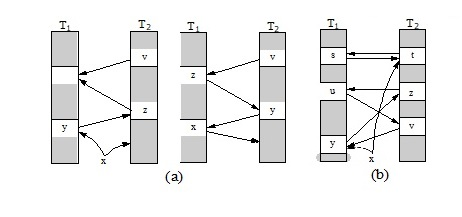
\includegraphics[scale=0.8]{hash_cuco.jpg}
\caption{ Ejemplos de inserci\'on de cuckoo Hashing. Las flechas muestran posibilidades para mover las teclas. (a) La clave x se inserta con éxito moviendo las teclas z e y de una tabla a la otra. (b) No se puede acomodar la llave x y es necesario un refrito.}
\label{fig 1}
\end{figure}
%%
\section{PRUEBA}
Ver en el cuaderno de jupyter en el siguiente enlace:  \url{https://github.com/crisebas/Cuckoo-Hashing/blob/master/experimentacion.ipynb}

%%BIBLIOGRAFIA
\begin{thebibliography}{}
\bibitem{}Rasmus, Pagh., Flemming Friche Rodler. (2001) Cuckoo Hashing. Journal of Algorithms.
\bibitem{}Samuel, Sánchez., Pablo, Domínguez., Luis Velásquez. (2009) Hashing: Técnicas y Hash para la
Protección de Datos. Universidad Tecnológica de Panamá.
\bibitem{}Mena Miranda, Yerko. (2009) Algoritmos HASH y vulnerabilidad a ataques. Universidad Mayor De San Andrés.
\bibitem{}Rasmus, Pagh. (2006) Cuckoo Hashing for Undergraduates. IT University of Copenhagen.



\end{thebibliography}
\end{document}
